% Audit d'ergonomie de ThesisManager (mod_these, mod_thesesynthesis) par acteur.
% Compilation : pdflatex audit-ergonomie-2026-10-26.tex (deux passes), paquets TeX Live
% latex-recommended, latex-extra, lang-french. Images : dossier images/ à côté de ce fichier.
\documentclass[11pt,a4paper]{article}
\usepackage[T1]{fontenc}
\usepackage[utf8]{inputenc}
\usepackage{lmodern}
\usepackage[french]{babel}
\usepackage[margin=2.2cm]{geometry}
\usepackage{booktabs}
\usepackage{longtable}
\usepackage{tabularx}
\usepackage{array}
\usepackage{enumitem}
\usepackage{xcolor}
\usepackage{graphicx}
\usepackage[colorlinks=true,linkcolor=blue!50!black,urlcolor=blue!50!black]{hyperref}

\setlist{nosep}
\sloppy
\setlength{\emergencystretch}{3em}
\newcommand{\code}[1]{\texttt{#1}}
\newcommand{\facile}{\textcolor{green!45!black}{\textbf{facile}}}
\newcommand{\moyen}{\textcolor{orange!80!black}{\textbf{moyen}}}
\newcommand{\difficile}{\textcolor{red!70!black}{\textbf{difficile}}}
\newcolumntype{Y}{>{\raggedright\arraybackslash}X}

\title{ThesisManager : audit d'ergonomie par acteur\\
  \large \code{mod\_these} 0.17.0 (2026102604) et \code{mod\_thesesynthesis} 0.5.0 (2026102600)}
\author{Sébastien Lefebvre}
\date{26 octobre 2026 --- serveur de test Moodle 4.5, PostgreSQL 16, PHP 8.3}

\begin{document}
\maketitle

\section*{Synthèse}

Le module est \textbf{facile} pour les acteurs qui agissent rarement et sur un seul objet
(membres du jury, signataires sans compte, agents DEVE, enseignants du suivi) : un lien ou une
page, une action. Il est \textbf{moyen} pour le directeur et la bibliothèque : le tableau de bord
dit quoi faire, mais chaque validation se fait sur une page très longue. Il est
\textbf{difficile} à deux moments : pour l'étudiant, le dépôt du dossier de soutenance (50 champs
sur six écrans) ; pour la DEVE, la validation du dossier de soutenance (44 champs, dix écrans) et
la navigation entre douze boutons et deux activités pour le paramétrage.

Les sept améliorations les plus rentables, par ordre d'effet :

\begin{enumerate}
  \item Pages de validation : mettre la décision \emph{après} le dossier, ou résumer le dossier au-dessus
    du formulaire ; aujourd'hui le dossier à examiner est \emph{sous} les boutons, à 6\,000--8\,000 pixels
    (§\ref{sec:transverse}).
  \item Bouton « Renvoyer le dossier » : le distinguer de « Valider » (secondaire, couleur d'alerte,
    commentaire obligatoire) ; les deux sont aujourd'hui des boutons principaux côte à côte.
  \item Dépôt du dossier de soutenance (étudiant) : découper en étapes ou indiquer l'avancement de
    chaque rubrique ; ne pas préremplir la date proposée avec l'heure courante.
  \item Écran d'accueil sur téléphone : la frise des onze étapes occupe tout le premier écran et
    repousse les actions ; la réduire à l'étape courante sur petit écran.
  \item Titre et description de l'activité affichés deux fois sur chaque page (en-tête Moodle et
    en-tête du module).
  \item Activité « Gestion des thèses » suivie : masquer (ou rediriger) les quatre boutons de
    paramétrage qui mènent à un simple renvoi vers l'activité de suivi.
  \item « Mes signatures » : ne pas cocher d'office tous les documents, les grouper par dossier et
    rappeler en tête, comme sur la page de signature, l'étudiant et le titre.
\end{enumerate}

\section{Méthode}

Serveur de test installé à partir de la branche de la version 0.17.0 (Moodle 4.5 sur
PostgreSQL 16, PHP 8.3), jeu de données des captures du guide
(\code{docs/guides/captures/seed.php}) : une promotion de 18 dossiers, chacun amené par le circuit
à une étape différente, de « sujet soumis » à « clos », une activité de suivi, un compte par
acteur. Un parcours automatisé (Playwright, Chromium) s'est connecté avec chaque compte et a ouvert
les 49 pages où l'acteur agit. Pour chaque page :

\begin{itemize}
  \item hauteur, exprimée en \emph{écrans} de 800 pixels (fenêtre de 1\,280 × 800) ;
  \item champs de saisie visibles, zones de dépôt de fichiers, boutons ;
  \item boutons visibles sans faire défiler, bouton principal ;
  \item débordement horizontal sur téléphone (390 pixels de large) ;
  \item erreurs PHP ou messages de débogage (aucun relevé) et textes restés en anglais.
\end{itemize}

Les écrans clés ont ensuite été examinés un à un. Les textes anglais relevés (« Save changes »,
« Back », « Expand all »\ldots) sont des chaînes du cœur de Moodle : le serveur de test n'a pas le
paquet de langue français. Ils seront traduits sur un site qui l'a installé ; ce n'est pas un
défaut du module.

Échelle : \facile{} (une page courte, action évidente depuis l'accueil), \moyen{} (action
trouvée sans aide mais page longue ou dense), \difficile{} (beaucoup de saisie, plusieurs
écrans, risque d'erreur ou de détour).

\section{Constats transverses}\label{sec:transverse}

\paragraph{Ce qui fonctionne bien.} Chaque acteur arrive sur une page qui dit quoi faire :
l'étudiant voit la frise des onze étapes, l'étape courante en bleu et « En attente : Étudiant »
ou le nom de l'acteur attendu ; le directeur, la bibliothèque et la DEVE ont un bloc « À traiter »
avec un bouton « Ouvrir ». Aucune erreur PHP sur les 49 pages ; aucun débordement horizontal
notable sur téléphone (3 pixels sur les tableaux de bord). Les actions rares et sensibles
(signature sur place, scan, renvoi) sont toutes inscrites à l'historique.

\paragraph{Pages de validation trop longues, décision avant le dossier.} Les pages « Valider
\ldots » placent le formulaire de décision en tête et le dossier complet en dessous :
6\,460 pixels pour la validation de la soutenance par le directeur, 7\,963 pour la DEVE, 6\,308 à
7\,885 pour la bibliothèque, alors que ces deux dernières ne saisissent souvent que 1 à 5 champs.
Le validateur doit descendre lire le dossier puis remonter décider. \emph{Proposition} : un résumé
du dossier (étudiant, titre, état, pièces) au-dessus du formulaire, le détail replié, ou la
décision en bas de page.

\paragraph{« Valider » et « Renvoyer le dossier » de même poids.} Les deux sont des boutons
principaux côte à côte (\code{review\_form}) ; un clic de travers renvoie le dossier.
\emph{Proposition} : « Renvoyer » en bouton secondaire ou d'alerte, avec commentaire
obligatoire et confirmation.

\paragraph{En-tête en double.} Le nom de l'activité et sa description apparaissent deux fois en
haut de chaque page (en-tête d'activité de Moodle 4, puis en-tête propre au module) : environ
200 pixels perdus, davantage sur téléphone.

\paragraph{Téléphone.} Sur 390 pixels, la frise des onze étapes occupe tout le premier écran de
l'étudiant ; les boutons d'action viennent après. \emph{Proposition} : sur petit écran, n'afficher
que « Étape 5/11 : Dépôt de la soutenance » et la frise repliée.

\begin{center}
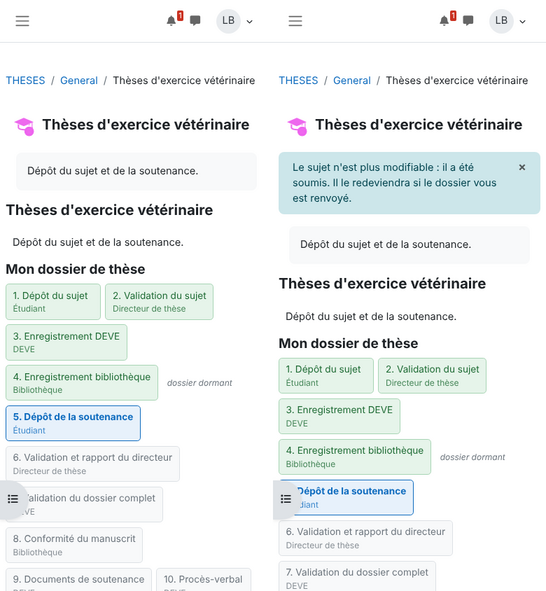
\includegraphics[width=0.75\linewidth]{images/audit-mobile-etudiant.png}\\
\small Accueil de l'étudiant et dépôt du sujet sur téléphone : frise et en-tête doublé avant toute action.
\end{center}

\paragraph{Signature tracée.} La première signature se trace à la souris ou au doigt ; aucune
alternative au clavier (accessibilité). La signature enregistrée évite de la retracer ensuite.
\emph{Proposition} : permettre, à défaut de tracé, une signature « nom tapé + certification »,
qui a la même valeur de signature électronique simple.

\section{Par acteur}

\subsection{Étudiant --- facile, sauf le dépôt de la soutenance (difficile)}

\begin{tabularx}{\linewidth}{@{}l Y c@{}}
\toprule
\textbf{Action} & \textbf{Constat} & \textbf{Niveau} \\
\midrule
Savoir où il en est & Frise des étapes, acteur attendu, date ; clair. & \facile \\
Déposer le sujet & 20 champs, une signature, 3 écrans ; brouillon possible. & \facile \\
Questionnaire & 6 champs, une page. & \facile \\
Déposer la soutenance & 50 champs, 2 dépôts de fichiers, 6 écrans : documents, date, jury
  ligne par ligne, identité, cursus, bordereau ABES, résumés, mots-clés, conclusions, contrat,
  signature. Brouillon possible mais aucune indication de ce qui reste à remplir ; date proposée
  préremplie avec l'heure courante, refusée seulement à l'envoi. & \difficile \\
Suivre un renvoi & Commentaire de renvoi en tête, en jaune ; clair. & \facile \\
Déposer les corrections & 1 fichier, une page. & \facile \\
\bottomrule
\end{tabularx}

\medskip
Trois boutons principaux de même poids à l'étape « Dossier actif » : « Questionnaire »,
« Déposer les documents de soutenance » et « Changer de sujet de thèse ». Le dernier, rare et
lourd de conséquences, gagnerait à être secondaire. Les pages d'accueil des étapes avancées
dépassent 6\,000 pixels (tout le dossier est affiché) ; des rubriques repliables aideraient.

\begin{center}
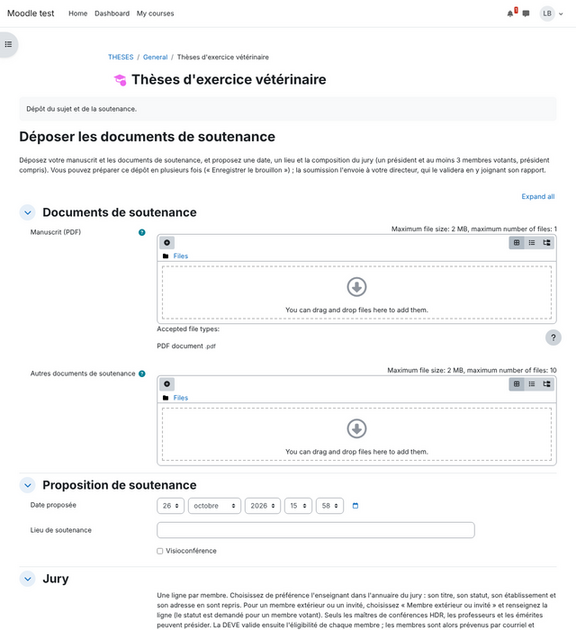
\includegraphics[width=0.6\linewidth]{images/audit-depot-soutenance.png}\\
\small Début du dépôt du dossier de soutenance : la première de six pages d'écran.
\end{center}

\subsection{Directeur de thèse --- moyen}

\begin{tabularx}{\linewidth}{@{}l Y c@{}}
\toprule
\textbf{Action} & \textbf{Constat} & \textbf{Niveau} \\
\midrule
Savoir quoi faire & « À traiter » en tête du tableau de bord (2 boutons de navigation). & \facile \\
Valider le sujet & 4 champs et une signature, mais 3 écrans (dossier sous le formulaire). & \facile \\
Valider la soutenance & Rapport, grille de conformité, agrément, signature : 27 champs, 8 écrans. & \moyen \\
Rapport seul & Page distincte (\code{report.php}) en plus de la validation : deux chemins pour le
  même rapport, à expliquer. & \moyen \\
Valider les corrections & 1 champ, mais 10 écrans de dossier. & \moyen \\
Planning & Ses soutenances, semaine ou mois ; clair. & \facile \\
\bottomrule
\end{tabularx}

\subsection{DEVE --- moyen, validation de la soutenance et paramétrage difficiles}

\begin{tabularx}{\linewidth}{@{}l Y c@{}}
\toprule
\textbf{Action} & \textbf{Constat} & \textbf{Niveau} \\
\midrule
Savoir quoi faire & « À traiter » (7 dossiers) puis tous les dossiers, filtres par statut ;
  efficace. Douze boutons de navigation sur deux lignes, 38 boutons sur la page. & \moyen \\
Enregistrer le sujet & 2 champs. & \facile \\
Valider la soutenance & N\textsuperscript{o} DEVE, date, lieu, jury ligne par ligne avec
  éligibilité, agrément : 44 champs, 10 écrans. L'avertissement de conflit de jury et celui du
  contrat type aident. & \difficile \\
Modifier un dossier & 31 champs, 4 écrans. & \moyen \\
Documents, signatures & Suivi des signatures : état par emplacement, relance, signature sur
  place en deux temps (identité puis signature) ; lisible. & \facile \\
Scan signé & Document, date, cases des signataires, fichier ; une page. & \facile \\
Procès-verbal, clôture & Depuis le dossier ; clôture : 1 champ, 10 écrans. & \moyen \\
Créer, importer & Pages courtes ; import CSV avec simulation. & \facile \\
Paramétrer & Réparti entre deux activités : dans « Gestion des thèses » suivie, Modèles,
  Grille, Questionnaire et Paramètres du circuit mènent à un renvoi vers le suivi (un clic
  perdu chacun). Paramètres du circuit : 18 champs sur 4 écrans ; grille : 66 champs, 7 écrans. & \difficile \\
\bottomrule
\end{tabularx}

\medskip
\emph{Propositions} : regrouper la navigation en deux menus (« Dossiers » : tableau de bord,
planning, création, import, export ; « Paramètres » : courriels, modèles, grille, questionnaire,
annuaire, paramètres du circuit, transfert) ; dans une activité suivie, remplacer les boutons de
paramétrage par un seul lien « Paramètres (activité de suivi) ».

\begin{center}
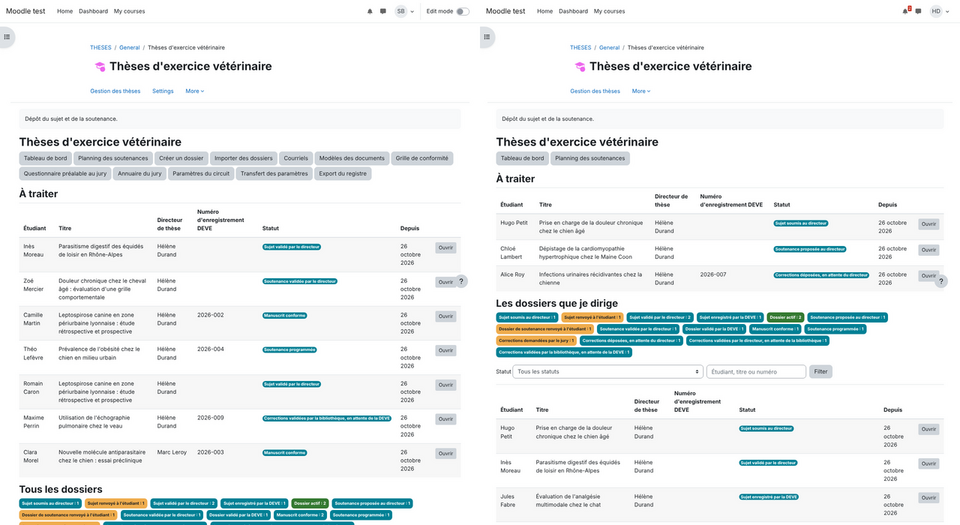
\includegraphics[width=0.95\linewidth]{images/audit-tableaux-de-bord.png}\\
\small Tableaux de bord de la DEVE (à gauche, douze boutons de navigation) et du directeur (à droite).
\end{center}

\subsection{Agent DEVE signataire --- facile}

Une page, « Mes signatures », toutes promotions confondues : documents, signature, un bouton.
Tous les documents sont \textbf{cochés d'office} : un agent peut signer sans avoir ouvert les PDF.
Les liens « voir le PDF » sont mal alignés quand le libellé passe à la ligne, et l'étudiant n'est
rappelé que par son nom. \emph{Propositions} : cases décochées, documents groupés par dossier avec
titre et n\textsuperscript{o} DEVE.

\subsection{Bibliothèque --- facile à moyen}

Tableau de bord avec « À traiter » (3 boutons de navigation). Notice du sujet : 2 champs ;
conformité : 5 champs ; corrections : 1 champ. Chaque page fait cependant 3 à 10 écrans, le
dossier étant affiché sous le formulaire (voir §\ref{sec:transverse}).

\subsection{Président du jury, direction, CCEM, université, directeur extérieur --- facile}

Un lien personnel reçu par courriel ouvre une page unique : document à signer présenté en tête
(qualité, étudiant, titre, n\textsuperscript{o} DEVE, soutenance, liens vers les PDF), tracé,
certification, un bouton. Sur place, la DEVE vérifie d'abord l'identité, puis la même page
s'ouvre. Un président qui a un compte retrouve aussi ses documents dans « Mes signatures ».

\subsection{Membre du jury --- facile}

Le lien d'accès ouvre une page sobre : étudiant, titre, date et lieu, composition du jury,
questionnaire, documents à télécharger. Rien à saisir.

\subsection{Enseignants (activité de suivi) --- facile}

« Suivi des thèses » (mes jurys) et « Rechercher des thèses » : une page chacune, 3 et 7 champs de
recherche.

\section{Mesures}

Hauteur en écrans de 800 pixels ; champs de saisie visibles ; zones de dépôt de fichiers ;
boutons visibles sur la page.

\begin{small}
\begin{longtable}{@{}p{3.1cm} p{6.4cm} r r r r@{}}
\toprule
\textbf{Acteur} & \textbf{Action} & \textbf{Écrans} & \textbf{Champs} & \textbf{Fich.} & \textbf{Boutons} \\
\midrule
\endhead
Étudiant & Accueil sans dossier & 1.0 & 0 & 0 & 1 \\
Étudiant & Déposer le sujet & 3.0 & 20 & 1 & 21 \\
Étudiant & Accueil, sujet en attente du directeur & 1.9 & 0 & 0 & 1 \\
Étudiant & Accueil, thèse en cours & 3.3 & 0 & 0 & 4 \\
Étudiant & Questionnaire préalable & 1.1 & 6 & 0 & 2 \\
Étudiant & Déposer le dossier de soutenance & 6.0 & 50 & 2 & 33 \\
Étudiant & Accueil, dossier renvoyé & 5.4 & 0 & 0 & 7 \\
Étudiant & Accueil, soutenance programmée & 7.9 & 0 & 0 & 7 \\
Étudiant & Accueil, corrections demandées & 8.8 & 0 & 0 & 8 \\
Étudiant & Déposer les corrections & 1.4 & 1 & 1 & 7 \\
Directeur & Accueil & 3.7 & 2 & 0 & 23 \\
Directeur & Tableau de bord & 3.7 & 2 & 0 & 23 \\
Directeur & Valider le sujet & 2.9 & 4 & 0 & 9 \\
Directeur & Rédiger le rapport & 2.1 & 2 & 1 & 9 \\
Directeur & Valider le dossier de soutenance & 8.1 & 27 & 0 & 16 \\
Directeur & Valider les corrections & 9.7 & 1 & 0 & 15 \\
Directeur & Planning & 1.8 & 2 & 0 & 10 \\
DEVE & Accueil & 4.4 & 2 & 0 & 38 \\
DEVE & Tableau de bord & 4.4 & 2 & 0 & 38 \\
DEVE & Dossier complet & 8.4 & 0 & 0 & 27 \\
DEVE & Enregistrer le sujet & 2.9 & 2 & 0 & 8 \\
DEVE & Valider le dossier de soutenance & 10.0 & 44 & 0 & 26 \\
DEVE & Modifier un dossier & 4.0 & 31 & 0 & 13 \\
DEVE & Documents générés & 1.8 & 0 & 0 & 2 \\
DEVE & Suivi des signatures & 2.7 & 0 & 0 & 19 \\
DEVE & Signature sur place (vérification) & 1.4 & 1 & 0 & 3 \\
DEVE & Déposer un scan signé & 1.7 & 7 & 1 & 8 \\
DEVE & Procès-verbal & 8.5 & 0 & 0 & 27 \\
DEVE & Clôturer (corrections conformes) & 10.2 & 1 & 0 & 16 \\
DEVE & Créer un dossier & 1.0 & 1 & 0 & 14 \\
DEVE & Importer des dossiers & 1.5 & 3 & 0 & 15 \\
DEVE & Courriels & 2.4 & 2 & 0 & 27 \\
DEVE & Annuaire du jury & 1.9 & 0 & 0 & 17 \\
DEVE & Transfert des paramètres & 2.2 & 14 & 0 & 18 \\
DEVE & Planning & 2.0 & 2 & 0 & 20 \\
DEVE (suivi) & Paramètres du circuit & 4.2 & 18 & 1 & 19 \\
DEVE (suivi) & Modèles des documents & 2.6 & 0 & 1 & 43 \\
DEVE (suivi) & Grille de conformité & 7.2 & 66 & 0 & 14 \\
DEVE (suivi) & Suivi des thèses & 5.1 & 3 & 0 & 35 \\
Agent DEVE & Mes signatures & 1.6 & 9 & 0 & 3 \\
Bibliothèque & Accueil & 3.8 & 2 & 0 & 25 \\
Bibliothèque & Tableau de bord & 3.8 & 2 & 0 & 25 \\
Bibliothèque & Enregistrer la notice (sujet) & 3.2 & 2 & 0 & 8 \\
Bibliothèque & Attester la conformité & 7.9 & 5 & 0 & 15 \\
Bibliothèque & Valider les corrections & 9.9 & 1 & 0 & 15 \\
Président (compte) & Mes signatures & 2.1 & 19 & 0 & 3 \\
Enseignant & Suivi des thèses & 1.2 & 3 & 0 & 4 \\
Enseignant & Rechercher des thèses & 1.3 & 7 & 0 & 5 \\
Membre du jury (lien) & Accès aux documents & 1.2 & 0 & 0 & 0 \\
\bottomrule
\end{longtable}
\end{small}

\section{Limites}

L'audit mesure la conception des écrans, pas le temps réel d'usage : il ne remplace pas une
séance d'observation avec un étudiant, un directeur et un agent de la DEVE. Les mesures ont été
prises sur un jeu de données de démonstration (titres courts, jury de quatre membres) ; un jury
de six membres allonge encore les pages de dépôt et de validation. Le serveur de test n'avait
pas le paquet de langue français de Moodle.

\end{document}
